\documentclass{article}
\usepackage{amsmath}
\usepackage{amssymb}
\usepackage{enumitem}
\usepackage{algorithm}
\usepackage{listings}
\usepackage{color,xcolor}
\usepackage[T1]{fontenc}
\usepackage{etoolbox}
\usepackage{multicol}
\usepackage{geometry}
\usepackage[colorlinks=true,linkcolor=blue,urlcolor=red,bookmarksopen=true]{hyperref}
\usepackage{tikz, pgfplots, tkz-euclide,calc}
    \usetikzlibrary{patterns,snakes,shapes.arrows,3d,patterns.meta,angles,quotes}
    \geometry{
        total = {160mm, 237mm},
        left = 25mm,
        right = 35mm,
        top = 30mm,
        bottom = 30mm,
      }

\usepackage{tcolorbox}
     \tcbuselibrary{listings,skins}

\newcommand{\enter}{\raisebox{-1.8pt}{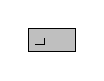
\begin{tikzpicture}[scale=0.3]
    \draw[thin,fill=lightgray] (0,0) rectangle (2,1);
    \draw (0.3,0.3) -- (0.7,0.3)--(0.7,0.6);     
\end{tikzpicture}}}

\definecolor{HIMAmuda}{HTML}{01D1FD}
\definecolor{HIMAtua}{HTML}{02016A}
\definecolor{HIMAabu}{HTML}{CBCBCC}
\definecolor{pgray}{rgb}{0.5,0.5,0.5}
\definecolor{pblue}{rgb}{0.13,0.13,1}
\definecolor{pgreen}{rgb}{0,0.5,0}
\definecolor{pred}{rgb}{0.9,0,0}
\definecolor{pgrey}{rgb}{0.46,0.45,0.48}
\definecolor{pcyan}{HTML}{D4EFFC}
\definecolor{lblue}{HTML}{00AEEF}
\definecolor{input}{HTML}{AAE1FA}
\definecolor{bg}{rgb}{0.95, 0.95, 0.92}
\definecolor{vscode}{HTML}{282A36}
\definecolor{PastelGreen}{HTML}{77DD77}

\newcommand{\inputscan}[1]{\raisebox{0pt}[1pt]{\colorbox{darkgray}{#1}}}

\usepackage{listings}

\lstdefinestyle{Liang}{
language=Java,
showspaces=false,
showtabs=false,
breaklines=true,
showstringspaces=false,
breakatwhitespace=true,
commentstyle=\color{pgray},
keywordstyle=\color{pblue},
stringstyle=\color{pgreen},
basicstyle=\small\ttfamily,
frame=single,
backgroundcolor=\color{pcyan},
escapeinside={(*}{*)},}

\lstdefinestyle{output}{
    language=Java,
    backgroundcolor=\color{vscode},
    basicstyle=\small\ttfamily\color{white},
    frame=none,
    escapeinside={(*}{*)},
    showspaces=false,
    showtabs=false,
    breaklines=true,
    showstringspaces=false,
    breakatwhitespace=true,
    keywordstyle=\color{white},
    }

\lstdefinestyle{standard}{
    language=Java,
    showspaces=false,
    showtabs=false,
    breaklines=true,
    showstringspaces=false,
    breakatwhitespace=true,
    commentstyle=\color{pgray},
    keywordstyle=\color{pblue},
    stringstyle=\color{pgreen},
    basicstyle=\small\ttfamily,
    frame=single,
    backgroundcolor=\color{bg},
    escapeinside={(*}{*)},}
\lstset{style=Liang}

\newtcblisting{RunCode}[1][enhanced,drop shadow]{
    arc=0pt, outer arc=0pt,
    boxsep=1pt,
    boxrule=2pt,
    auto outer arc,
    colback=vscode,
    colframe=bg,
    listing only, 
    listing style=output,
    title=\color{black}Ex. Output,
    #1
    }

\newtcolorbox{hint}[1][]{
    colback=PastelGreen!5!white, 
    colframe=PastelGreen!75!black,
    fonttitle=\bfseries, 
    colbacktitle=PastelGreen!85!black,
    enhanced, 
    attach boxed title to top left={yshift=-2mm}, 
    title=Hint,
    #1
}

\newtcolorbox{req}[1][]{
    colback=lblue!5!white, 
    colframe=lblue!75!black,
    fonttitle=\bfseries, 
    colbacktitle=lblue!85!black,
    enhanced, 
    attach boxed title to top left={yshift=-2mm}, 
    title=Input,
    #1
}

\newtcolorbox{out}[1][]{
    colback=HIMAtua!5!white, 
    colframe=HIMAtua!75!black,
    fonttitle=\bfseries, 
    colbacktitle=HIMAtua!85!black,
    enhanced, 
    attach boxed title to top left={yshift=-2mm}, 
    title=Output,
    before upper=\renewcommand\thempfootnote{\Roman{mpfootnote}},
    #1
}

\renewcommand{\thesubsection}{\arabic{subsection}}
\newcommand{\R}{\mathbb{R}}
\newcommand{\Z}{\mathbb{Z}}

\title{\textbf{Tugas Pertemuan 3}}
\date{26 September 2024}
\author{Dhanar A \& Fajar A}

\begin{document}
    \maketitle
    \pagenumbering{gobble}

    \section*{Problems}
    \begin{enumerate}[label=\textbf{\arabic*.}]
        %No 1
        \item \textbf{(Fisika)}\\
        Dengklek adalah seorang programmer di tim robotik ITS. Hari ini, dia diberi tanggung jawab untuk melakukan pengujian terhadap tembakan robot yang telah dirakit oleh tim mekanik. Dia diminta untuk mencari \textbf{jarak horizontal maksimum} yang dapat dicapai oleh tembakan robot, dengan memperhatikan beberapa batasan teknis yang ada. Dengklek mengandalkan ilmu Fisika 1 yang didapatkan selama kuliah untuk menghitung jarak tersebut \\
        \textit{ (Note : Aumsikan percepatan gravitasi $9.8$ $m/s^2$)} 
        \begin{req}
            \begin{itemize}
                \item \textbf{Kecepatan tangensial maksimum} roller robot tidak boleh lebih dari 30 m/s.
                \item \textbf{Sudut tembakan} robot adalah 45 derajat.
                \item Ada \textbf{kerugian kecepatan (losses)} akibat gesekan dan faktor lainnya, yaitu :
                \begin{enumerate}
                    \item Untuk kecepatan awal antara $1$ hingga $10$ $m/s$ , ada tambahan kecepatan sebesar $1$ $m/s$.
                    \item Untuk kecepatan awal antara $11$ hingga $20$ $m/s$, ada tambahan kecepatan sebesar $3$ $m/s$.
                    \item Untuk kecepatan awal antara $21$ hingga $30$ $m/s$, ada tambahan kecepatan sebesar $5$ $m/s$.
                \end{enumerate}
            \end{itemize}
        \end{req}

        \begin{out}
            \begin{itemize}
                \item $S:=$ Jarak horizontal maksimum \footnote{Cukup tampilkan 2 angka dibelakang koma}
                \item $S \geq 0, \quad S \in \R$
            \end{itemize}
        \end{out}   
        
        \begin{hint}
            Ubah sudut dari derajat ke radian menggunakan \texttt{Math.toRadians()} 
        \end{hint}

        \begin{RunCode}
Kecepatan awal : (*\inputscan{10.0} \enter*)
Kecepatan tangensial : (*\inputscan{11.0} \enter*)
Jarak horizontal maksimum : 12.35 meter
        \end{RunCode}
        
            
        \begin{RunCode}
Kecepatan awal : (*\inputscan{23.0} \enter*)
Kecepatan tangensial : (*\inputscan{28.0} \enter*)
Jarak horizontal maksimum : 80.00 meter
        \end{RunCode}

        \begin{RunCode}
Kecepatan awal : (*\inputscan{15.0} \enter*)
Kecepatan tangensial : (*\inputscan{18.0} \enter*)
Jarak horizontal maksimum : 33.06 meter
        \end{RunCode}
        
        
        \newpage
        %No 2
        \item \textbf{(Logika)} \\
        Misalkan Anda ingin membuat sebuah program untuk bermain lotere. Program ini secara acak akan menghasilkan nomor lotere yang terdiri dari dua digit, kemudian meminta pengguna untuk memasukkan nomor dua digit. Setelah itu, program akan menentukan apakah pengguna menang berdasarkan aturan berikut :
        \begin{enumerate}
            \item Jika nomor yang dimasukkan pengguna sama persis dengan nomor lotere yang dihasilkan, pengguna akan mendapatkan hadiah sebesar Rp50.000.000.
            \item Jika semua digit dalam nomor yang dimasukkan cocok dengan semua digit di nomor lotere, pengguna akan mendapatkan hadiah sebesar Rp10.000.000.
            \item Jika satu digit dalam nomor yang dimasukkan cocok dengan salah satu digit di nomor lotere, pengguna akan mendapatkan hadiah sebesar Rp5.000.000.
            \item Jika tidak memenuhi poin 1,2 dan 3 . Tampilkan pesan “Maaf, coba lagi”.
        \end{enumerate}

        \begin{hint}
            \begin{itemize}
                \item Gunakan \texttt{Math.random()} untuk nomer lotre nya.
                \item Gunakan operasi modulo \texttt{\%} untuk memisahkan inputan (Digit pertama dan kedua)
            \end{itemize}
        \end{hint}

        \begin{RunCode}
Masukkan 2 digit : (*\inputscan{2 2} \enter*)
Nomor Lotre : 22
Selamat anda mendapatkan hadiah sebesar Rp.50.000.000
        \end{RunCode}

        \newpage
        %No 3
        \item \textbf{(Geometri Analitik)}\\
        Buatlah program untuk menghitung jarak dari titik $(x_0,y_0)$ ke garis lurus $Ax+By+C=0$. Input dan Display menggunakan JOptionPane
        \begin{req}
            \begin{itemize}
                \item $0\leq x_0,y_0\leq 9,\quad x_0,y_0\in\Z$
                \item $0 \leq A,B,C\leq 9,\quad a,b,c\in\Z$
            \end{itemize}
        \end{req}
        \begin{out}
            \begin{itemize}
                \item $d:=$ Jarak titik ke garis\footnote{Cukup tampilkan 3 angka di belakang koma}\\
                $d\geq 0,\quad d\in\R$
            \end{itemize}      
        \end{out}
        \begin{hint}
            \begin{itemize}
                \item  Gunakan \texttt{Math.abs()} untuk menghitung nilai mutlak. 
                \item Gunakan operasi modulo \texttt{\%} untuk memisahkan input (Ratusan, Puluhan, Satuan) 
                \item Gunakan \texttt{Integer.ParseInt()} untuk mengubah inputan dari String menjadi integer 
                \item Gunakan \texttt{showMessageDialog()} untuk mendisplay output
            \end{itemize}
           
        \end{hint}
        \begin{RunCode}
Masukkan titik (x0,y0): (*\inputscan{1 2} \enter*) 
Masukkan koefisien garis (A,B,C): (*\inputscan{1 1 0} \enter*)
Jarak titik (1,2) ke garis adalah 2.121
        \end{RunCode} 

    \begin{figure}[h]
        \centering
        \includegraphics[width=0.5\linewidth]{Output.png}
    \end{figure}
    \end{enumerate}
\end{document}